This section will describe our proving technique, which is based on the principle of symbolic execution of transformation rules. The SyVOLT tool which implements this technique is described in Section~\ref{sec:prover_tool}.

\subsection{Proving Technique}
This section will describe the operation of our contract prover such that contracts are proven on all executions of a
DSLTrans transformation.

The contract prover we describe here is the engine of
the SyVOLT tool, which can currently be used to develop and verify DSLTrans transformations within the Eclipse~\cite{Lucio2015,syvoltTool,syvoltVideo} and MPS environments. Examples of contracts we have proved on the \FTP transformation are also presented.

\subsection{Contract Proving Overview}

Given a transformation written in the DSLTrans transformation language, our
contract proving technique can prove whether pre-\slash post-condition contracts will hold or
not hold on all executions of the transformation. If a contract holds, then whenever the pre-condition of the contract matches over an input model, then the post-condition of the contract will match over the corresponding output model.

  \begin{figure}[ht]
     \begin{center}
       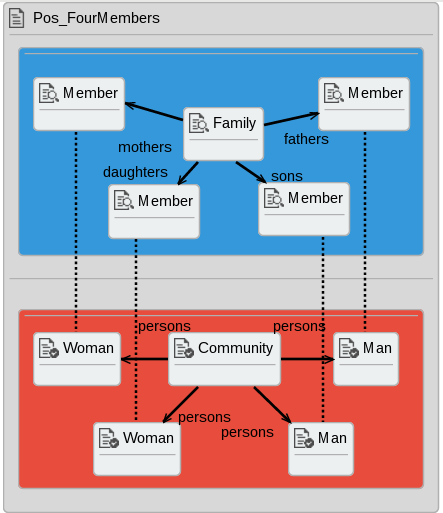
\includegraphics[width=0.36\textwidth]{figures/FamToPersons/Pos_FourMembers.png}
       \caption{A contract to verify that two \emph{Woman} and two \emph{Man} elements are produced from the corresponding \emph{Members}}
       \label{fig:familyProp}
     \end{center}
     \vspace{-0.15in}
   \end{figure}

For example, Figure~\ref{fig:familyProp} describes a contract to be proved over all transformation executions for the \FTP transformation. An informal statement for this contract is: \textit{`an input family with a father, mother, son and daughter should always produce
two men and two women in the output community'}.

Note that we employ backward links as part of the contract language, where as they are used to require that the output elements be generated from the attached input elements, similar to their use in DSLTrans rules. Our contract prover is then
able to prove whether or not this contract will hold for all transformation executions, and produce any counter-examples if they occur. Further examples of contracts are found in Section~\ref{sec:mbeddr_contracts} where we discuss contracts to be proved on our industrial case study.


 Contracts are proved through a process that first symbolically constructs all
 possible executions of the transformation, producing a set of \emph{path conditions}. Each path condition represents the execution of a set of transformation rules, by containing the input and output elements which are produced by the execution of those transformation rules.

 For example, the path condition in Figure~\ref{fig:pc_first} represents the execution of three rules in the transformation. This representation includes the input and output elements that will be present in the input and output models if these three rules execute. The set of path conditions produced by the prover will therefore partition the set of valid executions of the transformation, where each execution is an input/output model pair. This technique was first proposed in~\cite{Lucio2010} and further detailed in~\cite{Lucio2014}.

   \begin{figure}[t]
     \begin{center}
       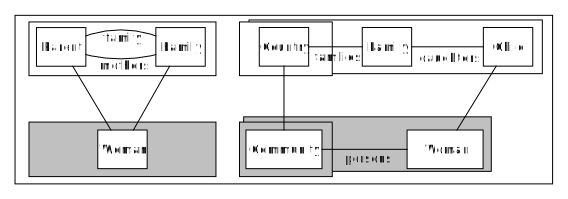
\includegraphics[width=0.45\textwidth]{figures/contract_proving/pc}
       \caption{An example path condition representing the execution of three rules}
       \label{fig:pc_first}
     \end{center}
     \vspace{-0.20in}
   \end{figure}

 Pre-/post-condition contracts form an implication, which needs to be checked
 for each path condition that has been generated by the proving algorithm. In broad
 terms, a contract holds on a path condition if either the contract's
 pre-condition elements cannot be found in the path condition, or the contract's pre-condition
 together with its post-condition can be found in the path condition. The contract
 does not hold on the path condition if its pre-condition can be
 found in the path condition but its post-condition cannot. Finally, a contract
 holds for a transformation if it holds for all of its generated path conditions.

 Contracts are formally described in~\cite{Lucio2014}, while extensive discussion of the contract language is found in the PhD thesis of Gehan Selim~\cite{Selim2015}. In addition, \cite{Oakes2016} briefly discusses the expressiveness of the contract language.

\subsection{Path Condition Creation}
\label{subsec:contract_prover}

As described in \cite{Lucio2015}, our contract prover constructs all artifacts used for contract proof through matching and rewriting of typed graphs. Therefore, the first step for the contract proving process is to create T-Core matcher and rewriter primitives from each of the rules
in the DSLTrans transformation~\cite{Syriani2013}. These model transformation primitives are at the core of our prover, allowing us to
reason about how rules could overlap with each other during transformation
execution, and to perform the graph rewriting necessary for our technique.

Note that this use of reasoning about the transformation under study as explicit graphs is in opposition to other approaches in the literature, where the transformation specifications are translated into a SAT solver or theorem prover, and then the proving mechanisms for those tools are used. A further discussion of our approach versus that in the literature can be found in~\cite{Selim2015}.

In order to fully reason about all input models to a transformation, our contract prover creates a set of artifacts that represent all
possible executions of the transformation. These artifacts are created by
symbolically executing all rules in the transformation, taking into account
rule overlapping and dependencies between rules. The rule combinations that are
created are termed \textit{path conditions}.

For example, the first path condition could represent the case where no rules in the transformation execute.
The next path condition is the case where only the first rule executes, the next
is where only the second rule executes, and a fourth path condition is where
both the two rules execute.

Note that in our path condition creation process, we
only consider one execution of each rule. That is, either a rule does not
execute (and does not appear in the path condition), or we assume that it executes some number of times (and the rule appears once). This restriction is due to our abstraction, where we symbolically represent
many executions of the same rule by the rule being present only once in each path
condition. This abstraction is necessary for analysis purposes, as the infinite number of transformation executions must be covered by a finite number of path conditions. Note that this abstraction is possible because of the
monotonicity of a DSLTrans transformation: a rule can only add elements to the
output model of a DSLTrans transformation, but never remove them.

As the transformation is made of layers, the symbolic execution process moves
through each layer and determines how rules may interact with each other. Unlike generating the powerset of all rules, these
rule interactions may in fact decrease the number of path conditions generated
by the prover as certain combinations of rules are proven infeasible. 

For example, consider a rule R1 which matches on an \textit{A} element, and a
rule R2 which matches on an \textit{A} element connected to a \textit{B}
element. During an execution of the transformation, it would be impossible for R2 to execute without R1 also executing, as the match graph of R1 is a subset of the match graph of R2. Therefore, the rule R1 is `subsumed' by the rule R2. Our prover is able to detect these subsumption interactions and resolve them in a step just prior to path condition generation. This lowers the number of path conditions created by disallowing certain rule combinations, as further discussed in~\cite{Selim2014}.

As well, DSLTrans rules can also define \textit{backward links}, as described for the extended \FTP transformation in Section~\ref{sec:background}. Recall that these backward links make dependencies on elements created by earlier rules. Specifically, these backward links require that the connected element in the apply part of the rule was created from the connected element in the match part of the rule, by matching over traceability links created during the execution of the transformation. During path condition construction, these backward link dependencies prevent some rules from executing, further decreasing the rule combinations possible.

More information on the specific cases of rule interactions can be found in~\cite{Oakes2016}.

\subsection{Contract Proving Process}
\label{subsub:contract_proving}

As path conditions are constructed through reasoning about the interaction of
transformation rules, the structure of a path condition is very similar to that
of a DSLTrans rule with a match graph and an apply graph, as seen in
Figure~\ref{fig:pc_first}.

The meaning of a particular path condition is, `if the elements in the top component of the path condition are in the input model, then the elements in the bottom component will be in the output model.' Recall that this matches the intended meaning of a contract: `if the elements in
the pre-condition are found in the transformation's input model, then the
post-condition elements should be found in the output model'. Therefore, to prove that a
contract holds or not on a path condition, it is sufficient to see whether the
elements in the contract can be matched onto the path condition, as described
in~\cite{Lucio2014}.


There are three cases for determining the status of a contract:
\begin{itemize}
\item If the pre-condition of the contract, including backward links, does not match the path condition, then the contract is not applicable for that path condition.
\item If both the pre-condition and post-condition match, then the contract does hold on that path condition.
\item If the pre-condition matches, but the post-condition does not match, then the contract does not hold on that path condition.
\end{itemize}

Note that a contract may be expected to not hold in all cases for a
transformation. For example, consider the contract \textit{Daughter\-Mother},
reproduced in Figure~\ref{fig:daughterMother}. The informal statement for this contract is `a family with a mother and a
daughter will always produce a community with a man'.  It is easy to see that an input model which contains only mother and
 daughter elements should not produce a man in the target community.

Our contract prover will then find multiple
 counter-example path conditions which cause the contract to not hold, such as the path condition in Figure~\ref{fig:pc_first}. Note that the
pre-condition of the contract does match onto the top component of the path condition, while the
\textit{Man} element in the contract post-condition cannot be found in the bottom component of the path condition. Thus the failure of this contract gives further
assurance that the transformation is working correctly, as \textit{daughters}
and \textit{mothers} are not accidentally transformed into \textit{men}. As this result is expected, this allows the transformation builder to have increased confidence in the validity of the transformation.


  \begin{figure}[t]
    \begin{center}
      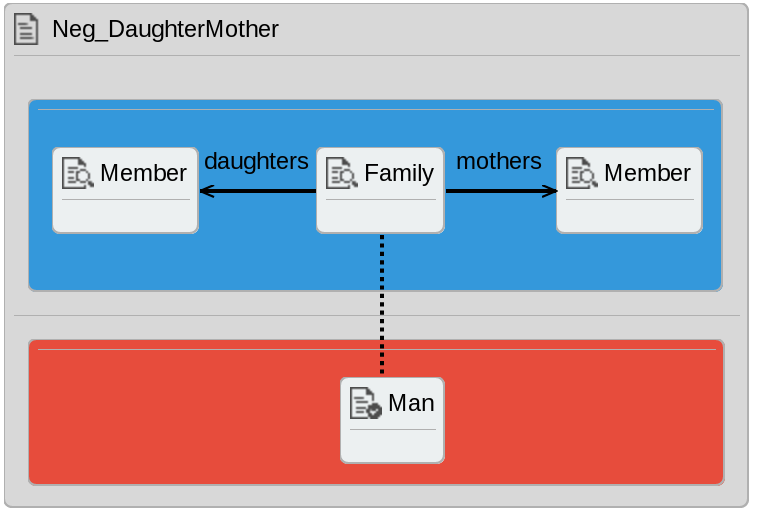
\includegraphics[width=0.45\textwidth]{figures/FamToPersons/Neg_DaughterMother}
      \caption{A contract to verify whether a \emph{Man} element will be produced from a \emph{Family} containing a \emph{daughter} element and a \emph{mother} element - this contract will not hold}
      \label{fig:daughterMother}
    \end{center}
    \vspace{-0.20in}
  \end{figure}

If a contract fails to hold on the transformation and it was not expected to fail, then this indicates an error with either the contract or the transformation. The prover will report (and optionally draw) the path conditions which the contract did not hold on. As well, a minimal path condition is reported, which represents the smallest combination of rules that fails. This allows the transformation developer to identify those rule combinations wherein an error may occur, and change the transformation or contract accordingly.

One of our research questions, as discussed in Section~\ref{sec:results}, asks whether we can further assist the user in determining the error given the path conditions where a problem arises. For example, our prover is able to identify contract elements which are not present in the transformation, preventing successful verification.


\subsubsection{Non-isomorphic Matching}
Note that, despite the fact that the pre-condition of the
\textit{Daughter\-Mother} contract cannot be (isomorphically) matched in the path
condition in Figure~\ref{fig:pc_first}, the pre-condition of the contract is still
found in that path condition. This is so because there are input models
matched by these two rules where the two distinct \textit{Family} elements
belonging to the two separate rules will match over the same family instance --
remember that in DSLTrans rules can match over the same elements in the input
model. The relation between the pre-condition of contracts and path condition is
thus such that, any possibility of overlaps (or absence thereof) between
elements of the same type belonging to two or more different rules in the path condition,
is considered as a matching possibility for the pre-condition of the
contract.

The relation between the contract and path condition packs thus more
information than a simple graph isomorphism. It is a mixed partial surjective /
injective homomorphism between the path condition and the contract typed graphs:
while the surjection allows ``forgetting'' that two or more elements in a path condition belong to
different rules, the injection guarantees that elements belonging to the
same rule in the path condition have an isomorphic counterpart in the property.
Further examples, as well as a formalization of this relation can be found in~\cite{Lucio2014}.

 In the case that the contract must explicitly reason about the multiplicity of \textit{Family} elements, the contract language includes
 propositional logic, as described in~\cite{Oakes2016}.





 